\chapter{Spintronique moléculaire}

\section{La spintronique}
La spintronique est une branche de l'électronique où, en plus de la charge, le degré de liberté du spin est utilisé. Elle est notamment à l'origine des avancés technologiques les plus récentes telle que la MRAM ou bien encore les têtes de lecture des disque durs. Une des applications les plus célèbre reste la vanne de spin. Ce dispositif permet de filtrer les électrons en fonction de l'orientation de leur spin (soit \textit{up}, soit \textit{down}), autorisant un couplage direct entre magnétisme et courant. La découverte du phénomène de magnétorésistance géante, à l'origine de ce filtrage, a d'ailleurs value à ces découvreurs, Albert Fert et Peter Grünberg, le prix Nobel de Physique en 2007.


Ces applications technologique restent cependant cantonnées au stockage de  l'information~\cite{Awschalom2007}. Des propositions de spin-transistor directement commandé par le spin de l'électron et non plus sa charge ont pourtant été faites~\cite{Datta1990} et certains dispositifs ont également été réalisé~\cite{Johnson1996,Huang2007}.

Cependant, l'électron n'est pas le seul objet possédant un spin et d'autre "acteurs" de la spintronique peuvent être envisagée. Les aimants moléculaire, notamment du fait de l'emmergence de l'électronique moléculaire, sont des candidats sérieux dans la fabrication de dispositifs toujours plus performants. Avant de voir comment ces derniers pourrait \^etre utilisés dans l'électronique de demain, nous allons définir ce qu'est réellement un aimant moléculaire et quelles sont ces caractéristiques.

\section{Les aimants moléculaires}
\subsection{Définition}

Un molécule, pour recevoir le qualificatif d'aimant, doit remplir deux critères. Tout d'abord, elle doit posséder un moment magnétique. Celui-ci résulte, en général, de l'interaction entre plusieurs centres magnétiques et donne lieux à un configuration où la résultante des moments magnétiques des différents centres est non nulle. 

Il faut en outre que ce moment magnétique ait une orientation préférentielle, le long de laquelle il va venir s'aligner. Les deux directions associées à cette orientation représente les deux configuration d'énergie minimale séparé par une barrière de potentiel. Afin qu'un aimant moléculaire conserve ses propriétés, il faut que l'énergie associé à l'agitation thermique soit plus faible que cette barrière. Dans le cas contraire, la température suffit à retourner aléatoirement le moment magnétique.

Certains aimants moléculaire, en plus de l'axe facile, possèdent également un plan difficile dans lequel l'énergie du moment magnétique est la plus grande. Cela donne naissance à une physique beaucoup plus riche de part l'apparition de phénomènes quantiques tels que le retournement de l'aimantation par effet tunnel~(QTM) ou bien encore la phase de Berry, que nous détaillerons dans la suite.

Malgré ces restrictions, la zoologie des aimants moléculaires est plutôt riche avec des moments magnétique allant de un à plusieurs dizaine $\mu_B$.


\subsection{Propriétés}
Les aimants moléculaires possèdent de nombreuses propriétés susceptibles de les rendre indispensable aux dispositifs électroniques de demain. Leur taille tout d'abord, en deçà des techniques lithographique, permettrait d'augmenter les densités de stockage, chaque molécule codant une information à travers l'orientation de son moment magnétique. Un telle application est notamment motivé par le faible taux de relaxation, de l'ordre de quelques années en dessous de $2\,K$, qui permettrait d'en faire des éléments de stockage de l'information fiable.

De plus, certains aimant moléculaires peuvent être sensible à un stimulus extérieur tels que la température, la lumières, la pression, un champ électrique ou magnétique ou bien encore un déplacement de charge. Ils peuvent ainsi osciller entre deux configurations magnétiques différentes : "haut spin" et "bas spin". Ces interrupteurs moléculaires pourraient également constituer le composant élémentaires des mémoires de demain.

Les aimants moléculaires peuvent également jouer un rôle non négligeable dans l'information quantique. Cette dernière vise à utiliser les propriétés des systèmes quantiques afin d'obtenir des algorithmes plus efficaces pour la factorisation des nombres premiers~(avec des applications dans la cryptographie notamment) ou bien encore la recherche dans les bases de données. Des phénomènes quantiques tels le QTM ou bien la phase de Berry pourrait être utilisé dans ce cadre.

Nous allons maintenant illustrer certaines de ces propriétés à travers l'exemple d'un aimant moléculaire bien connu le octanuclear fer(III) oxo-hydroxo cluster dont la formule est [Fe$_8$O$_2$(OH)$_{12}$(tacn)$_6$]$^{8+}$ ou Fe$_8$.

\subsection{L'exemple du Fe$_8$}

\begin{figure}
\centering 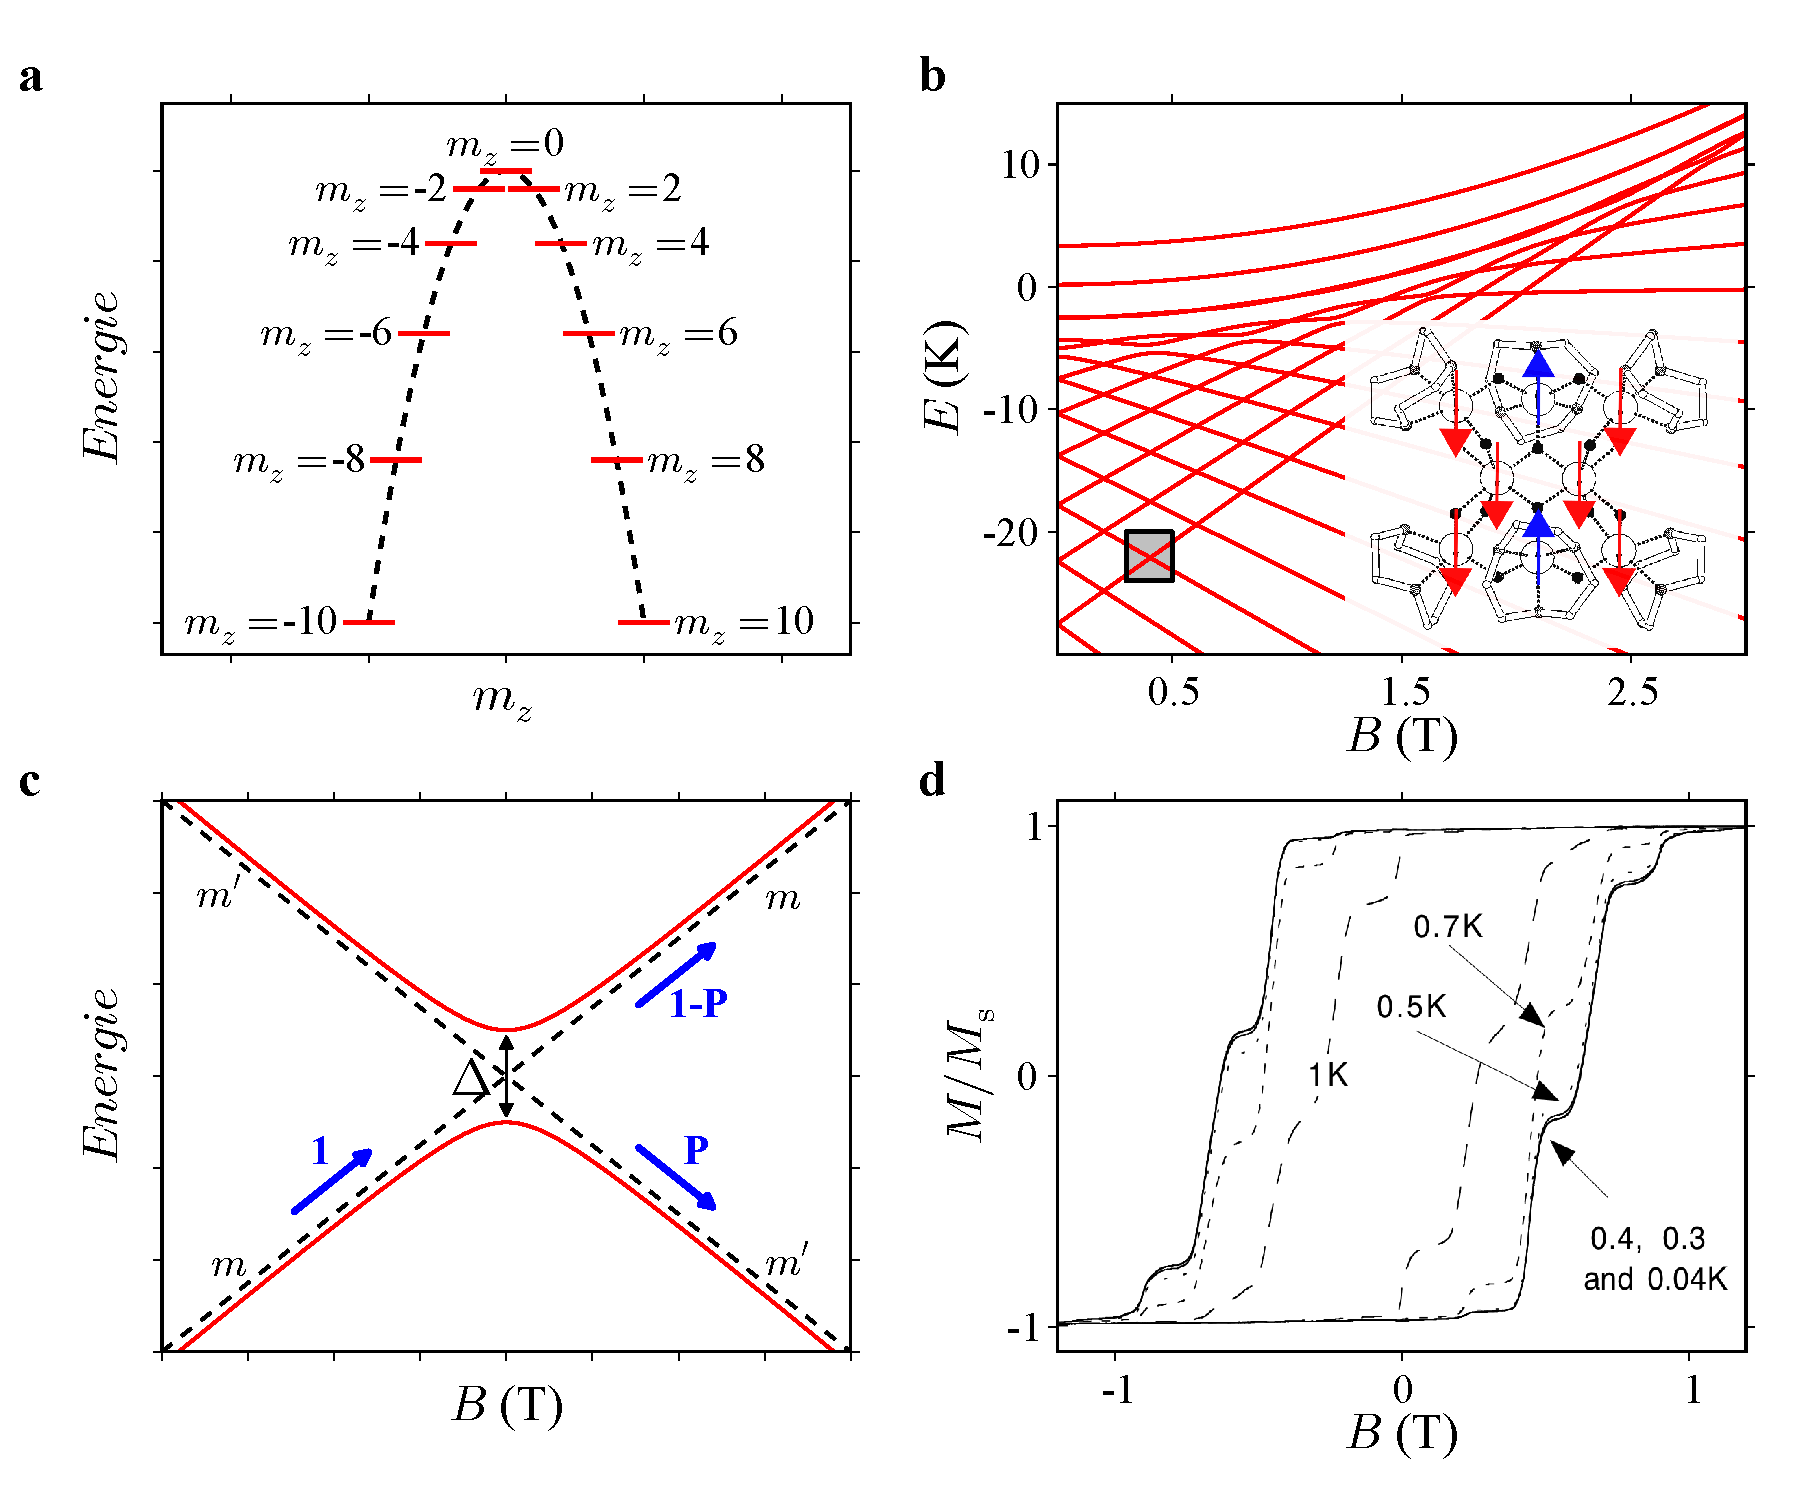
\includegraphics[scale=0.45]{Spintronique/FigureFe8/FigureFe8.pdf} 
\caption{\textbf{a} : énergie en fonction du nombre quantique $m_z$. Les deux orientations $m_z=\pm 10$ sont séparées par une barrière d'énergie de hauteur $|D|S^2$~\cite{Bogani2008}. \textbf{b} : diagramme Zeeman de la molécule Fe$_8$ représentant l'énergie des différents états du système en fonction du champ magnétique. Certains croisements, comme celui marqué d'un carré, sont en fait des anti-croisements traduisant un couplage entre les états. \textbf{c} : anti-croisement représentant un couplage entre les états $m$ et $m'$. \textbf{P} est la probabilité de transition entre les états $m$ et $m'$ lorsque l'on balaie l'anti-croisement en champ magnétique. \textbf{c} : mesure de l'aimantation d'un cristal de Fe$_8$ obtenue par technique micro-squid pour différentes températures. Les anti-croisements sont visibles à travers les marches qui traduisent un renversement de l'aimantation d'un grand nombre de molécules pour des valeurs particulières du champ magnétique~(extrait de \cite{MagGoesNano}).}
\label{Fe8Zeeman}
\end{figure}


Le Fe$_8$ se compose de huit atomes de fer de degré d'oxydation III, chacun de ces atomes constituant un centre magnétique de spin 5/2. De part les différentes interactions qui les lient, ils adoptent la configuration présenté dans la Fig.\ref{Fe8Zeeman}.\textbf{b} en encart avec un moment résultant total de $S=10$, le moment magnétique des deux atomes centraux se trouvant dans la direction opposée aux six atomes latéraux.

Les propriété magnétique de ce système peuvent \^etre décrite par l'hamiltonien suivant :
\begin{eqnarray}
E =  -DS_z^2 + \frac{E}{2} ( S_+^2  + S_-^2) + g\mu_b B S_z 
\end{eqnarray}
où $D$ est le paramètre d'anisotropie axiale, $E$ est le paramètre d'anysotropie transversale, $S_z$ et la projection sur $z$ du moment magnétique et $S_+$ et $S_-$ les opérateurs création anhilation.

\section{La spintronique moléculaire}
\subsection{État de l'art}
\subsection{La spintronique dans notre groupe}